For a general polynomial equation of degree 2,
\\
$p(x,y) \implies Ax^2+Bxy+Cy^2+Dx+Ey+F=0$
\\
The vector form is 
\begin{align}
\label{eq:5.2.1_vector_form}
\vec{x}^T \myvec{A & B/2\\B/2 & C}\vec{x}+ \myvec{D & E}\vec{x}+F=0
\end{align}
\begin{enumerate}
\item 
\begin{align}
y = x^2 - 1 &
\\
\implies \vec{x}^T \myvec{1 & 0\\0 & 0}\vec{x}+\myvec{0 & -1}\vec{x}-1&=0
\end{align}
For $\vec{x} = \myvec{1\\0}$,
\begin{align}
 \myvec{1 & 0}\myvec{1 & 0\\0 & 0} \myvec{1\\0}+\myvec{0 & -1}\myvec{1\\0}-1= 0
\end{align}
For $\vec{x} = \myvec{-1\\0}$,
\begin{align}
 \myvec{-1 & 0}\myvec{1 & 0\\0 & 0} \myvec{-1\\0}+\myvec{0 & -1}\myvec{1\\0}-1= 0
\end{align}
Hence +1,-1 are zeros, which can be verified from Fig. \ref{fig:5.2.1_parab1}
The python code for Fig. \ref{fig:5.2.1_parab1} is
\begin{lstlisting}
solutions/1/codes/conics/parab1.py
\end{lstlisting}
\begin{figure}[!ht]
\includegraphics[width=\columnwidth]{./solutions/1/figs/conics/parabola1.eps}
\caption{}
\label{fig:5.2.1_parab1}
\end{figure}
\item 
\begin{align}
y = \brak{x+1} \brak{x-2}&
\\
\implies \vec{x}^T \myvec{1 & 0\\0 & 0}\vec{x}+\myvec{-1 & -2}\vec{x}-2&=0
\end{align}
For $\vec{x} = \myvec{-1\\0}$,
\begin{align}
\myvec{-1 & 0} \myvec{1 & 0\\0 & 0}\myvec{-1\\0}+\myvec{-1 & -2}\vec{x}-2=0
\end{align}
Similarly, for 
For $\vec{x} = \myvec{2\\0}$,
\begin{align}
\myvec{2 & 0} \myvec{1 & 0\\0 & 0}\myvec{2\\0}+\myvec{-1 & -2}\vec{x}-2=0
\end{align}
Hence -1,+2 are zeros, which can be verified from Fig.  \ref{fig:5.2.1_parab2}
The python code  is
\begin{lstlisting}
solutions/1/codes/conics/parab2.py
\end{lstlisting}
\begin{figure}[!ht]
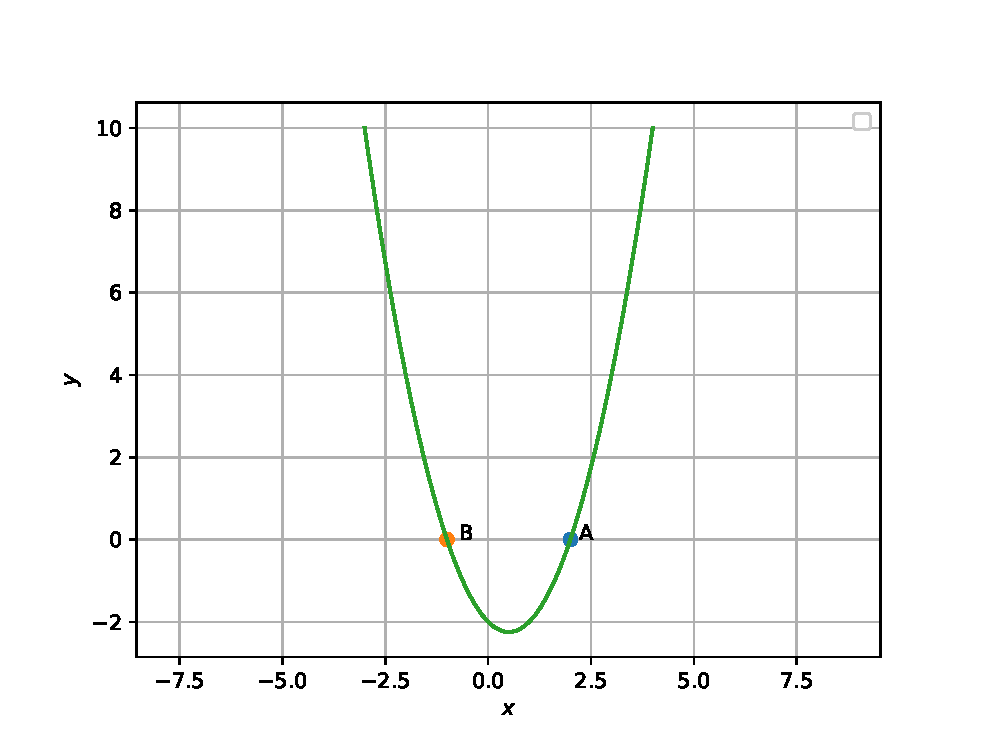
\includegraphics[width=\columnwidth]{./solutions/1/figs/conics/parabola2.eps}
\caption{}
\label{fig:5.2.1_parab2}
\end{figure}
\item 
\begin{align}
y = x^2 &
\\
\implies \vec{x}^T \myvec{1 & 0\\0 & 0}\vec{x}&=0
\end{align}
For $\vec{x} = \myvec{0\\0}$,
\begin{align}
\myvec{0 & 0} \myvec{1 & 0\\0 & 0}\myvec{0\\0}=0
\end{align}
Hence 0 is the  zero, which can be verified from the Fig.  \ref{fig:5.2.1_parab3}.
The python code is
\begin{lstlisting}
codes/conics/parab3.py
\end{lstlisting}
\begin{figure}[!ht]
\includegraphics[width=\columnwidth]{./solutions/1/figs/conics/parabola3.eps}
\caption{}
\label{fig:5.2.1_parab3}
\end{figure}
\item 
\begin{align}
y = 3x^2-1 &
\\
\implies \vec{x}^T \myvec{3 & 0\\0 & 0}\vec{x}+\myvec{0 & -1}\vec{x}-1&=0
\end{align}
For $\vec{x} = \myvec{-\frac{1}{\sqrt{3}}\\0}$,
\begin{align}
\myvec{-\frac{1}{\sqrt{3}} & 0}^T \myvec{3 & 0\\0 & 0}\myvec{-\frac{1}{\sqrt{3}}\\0}+\myvec{0 & -1}\myvec{-\frac{1}{\sqrt{3}}\\0}-1=0
\end{align}
For $\vec{x} = \myvec{\frac{2}{\sqrt{3}}\\0}$,
\begin{align}
\myvec{\frac{2}{\sqrt{3}} & 0}^T \myvec{3 & 0\\0 & 0}\myvec{\frac{2}{\sqrt{3}}\\0}+\myvec{0 & -1}\myvec{\frac{2}{\sqrt{3}}\\0}-1\ne 0
\end{align}
Hence $\frac{1}{\sqrt{3}}$ is a zero, but not $-\frac{2}{\sqrt{3}} $, which can be verified from Fig.  \ref{fig:5.2.1_parab4} generated through 
the python code 
\begin{lstlisting}
solutions/1/codes/conics/parab4.py
\end{lstlisting}
\begin{figure}[!ht]
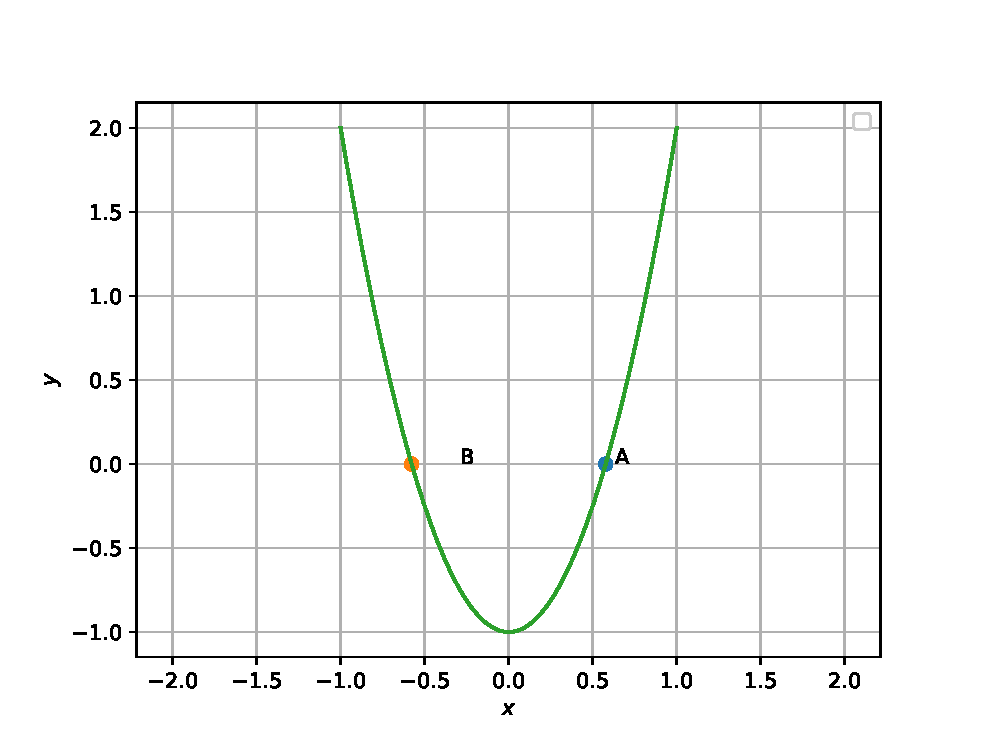
\includegraphics[width=\columnwidth]{./solutions/1/figs/conics/parabola4.eps}
\caption{}
\label{fig:5.2.1_parab4}
\end{figure}


\end{enumerate}
